\documentclass[11pt]{article}

% -------------------------------
% Paquetes
% -------------------------------
\usepackage[spanish]{babel}
\usepackage[utf8]{inputenc}
\usepackage{amsmath, amssymb}
\usepackage{graphicx}
\usepackage{booktabs}
\usepackage{geometry}
\usepackage[hypertexnames=false]{hyperref}
\usepackage{float}
\usepackage{caption}
\usepackage{subcaption}
\usepackage{fancyhdr}

\renewcommand{\thesubfigure}{\thefigure.\arabic{subfigure}}
\makeatletter
\renewcommand\p@subfigure{}
\makeatother
\DeclareCaptionLabelFormat{figurasub}{Figura~#2}
\captionsetup[subfigure]{labelformat=figurasub,labelsep=period}
\captionsetup[figure]{labelsep=period}

\graphicspath{{figures/}}

\geometry{margin=2.5cm}

\setlength{\parindent}{0pt}
\setlength{\parskip}{6pt}
\setlength{\headheight}{42pt}
\setlength{\headsep}{18pt}

\newcommand{\reportheader}{%
\begin{minipage}{\textwidth}
\vspace{6pt}
\makebox[\textwidth][s]{Trabajo Práctico N.º~2\hfill Series de Tiempo}
\vspace{6pt}
\hrule height 0.4pt
\end{minipage}%
}

\fancypagestyle{prismstyle}{%
  \fancyhf{}
  \fancyhead[C]{\reportheader}
  \fancyfoot[C]{\thepage}
  \renewcommand{\headrulewidth}{0pt}
  \renewcommand{\footrulewidth}{0pt}
}

\fancypagestyle{plain}{%
  \fancyhf{}
  \fancyhead[C]{\reportheader}
  \fancyfoot[C]{\thepage}
  \renewcommand{\headrulewidth}{0pt}
  \renewcommand{\footrulewidth}{0pt}
}

\pagestyle{prismstyle}

% -------------------------------
% Título
% -------------------------------
\title{%
\textbf{Elasticidades del comercio exterior argentino} \\
\large \textbf{Trabajo Práctico N° 2 - Series de Tiempo}
}

\author{
\textbf{Maestría en Economía Aplicada} \\
\textbf{Facultad de Ciencias Económicas - UBA} \\
\\
\textbf{Integrantes:} \\
Andrea Chasi \\
Julián Delgadillo Marín \\
Christian Arias \\
Leonardo Ávila \\
\\
\textbf{Docente:} \\
Julio Eduardo Fabris
}

\date{\textbf{Fecha de entrega:} 26 de mayo de 2026}

\begin{document}

\maketitle

% -------------------------------
% Resumen
% -------------------------------
\begin{abstract}
\label{sec:abstract}
resumen del trabajo abstract
\end{abstract}

% -------------------------------
% 1. Introducción
% -------------------------------
\section{Introducción}
\label{sec:introduccion}



% -------------------------------
% 2. Marco metodológico
% -------------------------------
\section{Marco metodológico}
\label{sec:marco-metodologico}

El trabajo estima elasticidades de largo y corto plazo del comercio exterior
argentino mediante modelos en logaritmos, pruebas de integración,
cointegración y modelos dinámicos. Todas las variables reales se transforman a
logaritmos naturales según la ecuación \eqref{eq:transformacion-logaritmica}.
Esta decisión permite interpretar los coeficientes de las relaciones en niveles
como elasticidades. Las variaciones trimestrales se aproximan mediante primeras
diferencias logarítmicas, definidas en la ecuación
\eqref{eq:primera-diferencia-logaritmica}.

\begin{equation}
z_t = \ln(Z_t)
\label{eq:transformacion-logaritmica}
\end{equation}

\begin{equation}
\Delta z_t = z_t - z_{t-1}
\label{eq:primera-diferencia-logaritmica}
\end{equation}

Para representar la demanda externa relevante de las exportaciones argentinas,
se construye un indicador de PIB de socios comerciales a partir de los PIB de
Brasil y Estados Unidos. La agregación se realiza como combinación ponderada en
logaritmos, de acuerdo con la ecuación \eqref{eq:pib-socios}, donde los pesos
\(w_{BR}\) y \(w_{US}\) provienen de la estructura de ponderadores utilizada en
el índice de tipo de cambio real multilateral.

\begin{equation}
\ln(PIBSOCIOS_t)
= w_{BR}\ln(PIB_{BR,t}) + w_{US}\ln(PIB_{US,t})
\label{eq:pib-socios}
\end{equation}

La especificación de largo plazo para importaciones relaciona las importaciones
reales con el nivel de actividad local y el tipo de cambio real multilateral,
como se muestra en la ecuación \eqref{eq:largo-plazo-importaciones}. En esta
ecuación, \(\alpha_1\) mide la elasticidad ingreso de las importaciones y
\(\alpha_2\) mide la elasticidad frente al ITCRM.

\begin{equation}
\ln(M_t)
= \alpha_0 + \alpha_1 \ln(PIB_t) + \alpha_2 \ln(ITCRM_t) + u_t
\label{eq:largo-plazo-importaciones}
\end{equation}

Para exportaciones, la relación de largo plazo vincula las exportaciones reales
con el PIB de socios comerciales y el ITCRM, según la ecuación
\eqref{eq:largo-plazo-exportaciones}. En este caso, \(\gamma_1\) resume la
elasticidad respecto a la demanda externa y \(\gamma_2\) la respuesta frente al
tipo de cambio real.

\begin{equation}
\ln(X_t)
= \gamma_0 + \gamma_1 \ln(PIBSOCIOS_t) + \gamma_2 \ln(ITCRM_t) + v_t
\label{eq:largo-plazo-exportaciones}
\end{equation}

Antes de estimar modelos dinámicos, se evalúa el orden de integración de las
series mediante pruebas ADF, Phillips-Perron y KPSS. Luego se aplican pruebas
de cointegración de Engle-Granger sobre las relaciones de largo plazo. Para la
ecuación de importaciones, el residuo estimado se define en
\eqref{eq:residuo-engle-granger-importaciones}. Si este residuo es
estacionario, las variables comparten una relación de equilibrio de largo
plazo.

\begin{equation}
\widehat{u}_t
= \ln(M_t) - \widehat{\alpha}_0
- \widehat{\alpha}_1 \ln(PIB_t)
- \widehat{\alpha}_2 \ln(ITCRM_t)
\label{eq:residuo-engle-granger-importaciones}
\end{equation}

Cuando existe evidencia de cointegración, se estima un modelo de corrección del
error. Para importaciones, el modelo utilizado se resume en la ecuación
\eqref{eq:ecm-importaciones}. El término \(\widehat{u}_{t-1}\) representa el
desvío rezagado respecto del equilibrio de largo plazo, mientras que
\(\lambda\) mide la velocidad con la que el sistema corrige dicho desequilibrio.

\begin{equation}
\Delta \ln(M_t)
= \beta_0
+ \beta_1 \Delta \ln(PIB_t)
+ \beta_2 \Delta \ln(ITCRM_t)
+ \lambda \widehat{u}_{t-1}
+ \sum_{j=1}^{p}\phi_j \Delta \ln(M_{t-j})
+ \varepsilon_t
\label{eq:ecm-importaciones}
\end{equation}

La velocidad trimestral de ajuste se calcula como el valor absoluto del
coeficiente del término de corrección del error, multiplicado por cien, según
\eqref{eq:velocidad-ajuste}. En la estimación final de importaciones, el
coeficiente estimado implica una velocidad de ajuste de 32.9\%, como se muestra
en \eqref{eq:velocidad-ajuste-estimada}.

\begin{equation}
\text{Velocidad de ajuste trimestral}
= |\widehat{\lambda}| \times 100
\label{eq:velocidad-ajuste}
\end{equation}

\begin{equation}
|\widehat{\lambda}| \times 100 = |-0.329| \times 100 = 32.9\%
\label{eq:velocidad-ajuste-estimada}
\end{equation}

Cuando no se encuentra evidencia suficiente de cointegración, la especificación
se estima en primeras diferencias. Este es el caso de exportaciones, cuyo
modelo de corto plazo incorpora el crecimiento del PIB de socios, el ITCRM y el
índice de commodities, como se presenta en la ecuación
\eqref{eq:diferencias-exportaciones}.

\begin{equation}
\Delta \ln(X_t)
= \delta_0
+ \delta_1 \Delta \ln(PIBSOCIOS_t)
+ \delta_2 \Delta \ln(ITCRM_t)
+ \delta_3 \Delta \ln(COM_t)
+ \sum_{j=1}^{p}\psi_j \Delta \ln(X_{t-j})
+ \eta_t
\label{eq:diferencias-exportaciones}
\end{equation}

La cantidad de rezagos de los modelos dinámicos se selecciona mediante el
criterio de información bayesiano, definido en la ecuación \eqref{eq:bic}. Este
criterio penaliza la complejidad del modelo a través del número de parámetros
\(k_p\) y favorece especificaciones parsimoniosas.

\begin{equation}
BIC(p) = -2\ln(\widehat{L}_p) + k_p \ln(T)
\label{eq:bic}
\end{equation}

Como contraste adicional de robustez, se considera la posibilidad de quiebres
estructurales mediante la prueba de Gregory-Hansen. La ecuación
\eqref{eq:dummy-gregory-hansen} representa la variable indicadora asociada al
punto de quiebre \(\tau\), que permite evaluar si la relación de largo plazo
cambia a partir de una fecha determinada.

\begin{equation}
D_t(\tau) =
\begin{cases}
0, & t \leq [T\tau] \\
1, & t > [T\tau]
\end{cases}
\label{eq:dummy-gregory-hansen}
\end{equation}



% -------------------------------
% 3. Datos
% -------------------------------
\section{Datos}
\label{sec:datos}

La base empírica del trabajo reúne series trimestrales del comercio exterior
argentino, actividad económica local, demanda externa, tipo de cambio real y
precios internacionales de commodities. La construcción de la base busca
mantener una muestra homogénea para las estimaciones econométricas y, al mismo
tiempo, documentar la cobertura disponible de cada fuente.

\subsection{Fuentes y construcción de variables}
\label{subsec:fuentes-construccion-variables}

Las variables de comercio exterior y el PIB de Argentina provienen de fuentes
oficiales nacionales, mientras que las variables externas se construyen a
partir de información internacional y del BCRA. Todas las series se expresan en
frecuencia trimestral y se transforman a logaritmos naturales y primeras
diferencias logarítmicas para el análisis econométrico. El Cuadro
\ref{tab:variables-fuentes-transformaciones} resume las fuentes, la cobertura
disponible y las transformaciones aplicadas.

El índice de commodities se incorpora como variable externa adicional para
capturar shocks de precios internacionales relevantes para las exportaciones
argentinas. En la especificación final no se utiliza como determinante de la
relación de largo plazo, sino como regresor de corto plazo en el modelo en
primeras diferencias de exportaciones.

El PIB de socios comerciales se construye como un índice ponderado de Brasil y
Estados Unidos. Los ponderadores provienen de la estructura utilizada por el
BCRA para el ITCRM, por lo que reflejan la importancia relativa de cada socio en
el comercio argentino. Como el indicador se limita a estos dos países, los pesos
originales se normalizan para que sumen 100\%. Así, Brasil recibe una
participación mayor por su peso relativo dentro del comercio argentino, mientras
que Estados Unidos completa el índice como segundo socio considerado. El Cuadro
\ref{tab:ponderadores-pib-socios} presenta los pesos utilizados y la Figura
\ref{fig:cobertura-temporal-series} muestra la cobertura temporal de las series
principales.

\begin{table}[H]
\centering
\caption{Variables, fuentes, cobertura y transformaciones de la base de datos.}
\label{tab:variables-fuentes-transformaciones}
\small
\begin{tabular}{p{3.1cm}p{4.1cm}p{2.0cm}p{2.4cm}p{4.3cm}}
\toprule
Variable & Fuente & Frecuencia & Cobertura disponible & Transformación aplicada \\
\midrule
Importaciones reales & INDEC, comercio exterior y cuentas nacionales & Trimestral & 2004Q1--2022Q4 & Logaritmo natural y primera diferencia logarítmica \\
Exportaciones reales & INDEC, comercio exterior y cuentas nacionales & Trimestral & 2004Q1--2022Q4 & Logaritmo natural y primera diferencia logarítmica \\
PIB Argentina & INDEC, cuentas nacionales & Trimestral & 2004Q1--2022Q4 & Logaritmo natural y primera diferencia logarítmica \\
PIB socios & FRED; ponderadores BCRA del ITCRM para Brasil y Estados Unidos & Trimestral & 2004Q1--2025Q4 & Índice ponderado, logaritmo natural y primera diferencia logarítmica \\
ITCRM & BCRA, índice de tipo de cambio real multilateral & Trimestral & 2004Q1--2025Q4 & Promedio trimestral, logaritmo natural y primera diferencia logarítmica \\
Commodities & Banco Mundial, Pink Sheet, índice agregado de commodities & Trimestral & 2004Q1--2025Q4 & Promedio trimestral, logaritmo natural y primera diferencia logarítmica \\
\bottomrule
\end{tabular}
\end{table}

\begin{table}[H]
\centering
\caption{Ponderadores utilizados para construir el PIB de socios comerciales.}
\label{tab:ponderadores-pib-socios}
\small
\begin{tabular}{p{3.0cm}p{3.0cm}p{3.0cm}p{3.0cm}p{3.8cm}}
\toprule
País & Variable fuente & Ponderador BCRA & Ponderador normalizado & Período de ponderación \\
\midrule
Brasil & brasil & 32.19 & 71.07\% & 2004-01--2025-12 \\
Estados Unidos & estados\_unidos & 13.10 & 28.93\% & 2004-01--2025-12 \\
\bottomrule
\end{tabular}
\end{table}

\begin{figure}[H]
\centering

\includegraphics[width=\textwidth]{section_08_data_coverage.png}
\caption{Cobertura temporal de las series principales.}
\label{fig:cobertura-temporal-series}
\end{figure}

\subsection{Evolución descriptiva de las series}
\label{subsec:evolucion-descriptiva-series}

La inspección gráfica permite identificar la dinámica general de las variables
antes de avanzar hacia las pruebas econométricas. En la ecuación de
importaciones, la Figura \ref{fig:logs-importaciones} muestra la evolución de
las importaciones reales, el PIB de Argentina y el ITCRM en logaritmos. Las
importaciones y el nivel de actividad local presentan movimientos persistentes
en el tiempo, con episodios de caída asociados a períodos de contracción
macroeconómica. El ITCRM, por su parte, exhibe cambios de nivel y oscilaciones
que justifican tratarlo como una variable relevante para la dinámica comercial.

\begin{figure}[H]
\centering

\includegraphics[width=\textwidth]{section_08_imports_logs.png}
\caption{Series en logaritmos de importaciones reales, PIB de Argentina e ITCRM.}
\label{fig:logs-importaciones}
\end{figure}

Para exportaciones, la Figura \ref{fig:logs-exportaciones} presenta las series
en logaritmos asociadas a la demanda externa y a los precios internacionales.
Las exportaciones reales muestran una trayectoria menos regular que las
importaciones, mientras que el PIB de socios mantiene una tendencia creciente
más suave. El índice de commodities registra ciclos marcados, lo que respalda
su inclusión como variable externa para capturar shocks de precios
internacionales en el modelo de corto plazo.

\begin{figure}[H]
\centering

\includegraphics[width=\textwidth]{section_08_exports_logs.png}
\caption{Series en logaritmos de exportaciones reales, PIB de socios comerciales e índice de commodities.}
\label{fig:logs-exportaciones}
\end{figure}

Las Figuras \ref{fig:crecimiento-comercio-actividad} y
\ref{fig:crecimiento-variables-externas} muestran las primeras diferencias
logarítmicas expresadas como crecimientos trimestrales aproximados. Estas
transformaciones reducen la persistencia observada en los niveles y permiten
comparar la volatilidad de corto plazo entre comercio, actividad local,
demanda externa, ITCRM y commodities. En particular, las series de comercio y
commodities presentan fluctuaciones más pronunciadas que el PIB de socios, lo
que anticipa la necesidad de modelos dinámicos con rezagos y errores estándar
robustos.

\begin{figure}[H]
\centering

\includegraphics[width=\textwidth]{section_08_trade_growth.png}
\caption{Crecimiento trimestral aproximado del comercio y la actividad local.}
\label{fig:crecimiento-comercio-actividad}
\end{figure}

\begin{figure}[H]
\centering

\includegraphics[width=\textwidth]{section_08_external_growth.png}
\caption{Crecimiento trimestral aproximado de las variables externas.}
\label{fig:crecimiento-variables-externas}
\end{figure}

% -------------------------------
% 4. Resultados
% -------------------------------
\section{Resultados}
\label{sec:resultados}

Esta sección presenta los resultados econométricos del trabajo. El análisis
avanza desde la caracterización preliminar de las series hacia las pruebas de
cointegración, la estimación de elasticidades y los modelos dinámicos de corto
plazo. Esta secuencia permite distinguir entre relaciones de largo plazo
válidas y especificaciones que deben estimarse únicamente en primeras
diferencias.

\subsection{Análisis preliminar de las series}
\label{subsec:analisis-preliminar-series}

El primer paso consiste en evaluar las propiedades temporales de las variables
utilizadas en las ecuaciones de importaciones y exportaciones. Dado que el
trabajo combina modelos en niveles y en primeras diferencias, es necesario
identificar si las series presentan raíces unitarias y si las transformaciones
aplicadas producen variables estacionarias. El Cuadro
\ref{tab:raiz-unitaria-estacionariedad} resume los resultados de las pruebas
ADF, Phillips-Perron y KPSS para las variables principales.

\begin{table}[H]
\centering
\caption{Pruebas de raíz unitaria y estacionariedad.}
\label{tab:raiz-unitaria-estacionariedad}
\small
\resizebox{\textwidth}{!}{%
\begin{tabular}{lccccccc}
\toprule
Variable & ADF nivel & PP nivel & KPSS nivel & ADF dif. & PP dif. & KPSS dif. & Decisión final \\
\midrule
Importaciones reales & 0.232 & 0.588 & 0.010 & 0.017 & 0.010 & 0.100 & I(1) \\
Exportaciones reales & 0.045 & 0.010 & 0.019 & 0.010 & 0.010 & 0.100 & I(1) \\
PIB Argentina & 0.199 & 0.024 & 0.010 & 0.010 & 0.010 & 0.090 & I(1) \\
PIB socios & 0.583 & 0.663 & 0.010 & 0.014 & 0.010 & 0.100 & I(1) \\
ITCRM & 0.714 & 0.725 & 0.010 & 0.010 & 0.010 & 0.100 & I(1) \\
Commodities & 0.334 & 0.488 & 0.017 & 0.030 & 0.010 & 0.100 & I(1) \\
\bottomrule
\end{tabular}%
}
\end{table}

Los resultados sugieren que las variables principales pueden tratarse como
integradas de orden uno. En términos prácticos, esto justifica trabajar con
primeras diferencias para capturar la dinámica de corto plazo y, al mismo
tiempo, evaluar si existen relaciones de cointegración que permitan estimar
modelos de corrección del error.

Además de la integración, se revisa la presencia de patrones estacionales en
las primeras diferencias logarítmicas. El Cuadro
\ref{tab:diagnostico-estacionalidad} muestra que las variables de comercio y el
PIB de Argentina presentan evidencia compatible con estacionalidad, mientras
que ITCRM, PIB socios y commodities no muestran evidencia estadística al 5\%.
La decisión metodológica es no aplicar un ajuste estacional adicional, sino
controlar la dinámica mediante diferencias logarítmicas y rezagos en los
modelos estimados.

\begin{table}[H]
\centering
\caption{Diagnóstico de estacionalidad en primeras diferencias logarítmicas.}
\label{tab:diagnostico-estacionalidad}
\small
\resizebox{\textwidth}{!}{%
\begin{tabular}{lrrll}
\toprule
Serie & p-value & Evidencia al 5\% & Serie afectada & Decisión metodológica \\
\midrule
Importaciones reales & $<0,001^{***}$ & Posible patrón estacional & Sí & No se ajusta; se controla con diferencias y rezagos \\
Exportaciones reales & $<0,001^{***}$ & Posible patrón estacional & Sí & No se ajusta; se controla con diferencias y rezagos \\
PIB Argentina & $<0,001^{***}$ & Posible patrón estacional & Sí & No se ajusta; se controla con diferencias y rezagos \\
ITCRM & 0.337 & Sin evidencia estadística & No & Sin ajuste estacional adicional \\
PIB socios & 0.881 & Sin evidencia estadística & No & Sin ajuste estacional adicional \\
Commodities & 0.439 & Sin evidencia estadística & No & Sin ajuste estacional adicional \\
\bottomrule
\end{tabular}%
}
\vspace{1mm}

\begin{minipage}{0.96\textwidth}
\footnotesize \textit{Nota:} *, ** y *** indican rechazo de la hipótesis nula al 10\%, 5\% y 1\%, respectivamente.
\end{minipage}
\end{table}

\subsection{Cointegración y elasticidades de largo plazo}
\label{subsec:cointegracion-elasticidades-largo-plazo}

Una vez establecida la naturaleza integrada de las series, se evalúa si las
variables de cada ecuación comparten una relación de equilibrio de largo plazo.
Para ello se aplican pruebas de cointegración de Engle-Granger y
Gregory-Hansen. La primera contrasta la estacionariedad de los residuos de las
ecuaciones de largo plazo, mientras que la segunda permite considerar la
presencia de un quiebre estructural en la relación estimada.

El Cuadro \ref{tab:pruebas-cointegracion} muestra que la ecuación de
importaciones presenta evidencia suficiente de cointegración. El estadístico de
Engle-Granger es menor que el valor crítico al 5\% y la prueba de
Gregory-Hansen también respalda la existencia de una relación de largo plazo
con quiebre. Por este motivo, la especificación de importaciones se estima
luego mediante un modelo de corrección del error. En cambio, para
exportaciones la evidencia no resulta suficientemente robusta: aunque el
p-value aproximado de Engle-Granger es bajo, la comparación con los valores
críticos de la prueba y el contraste con quiebre no sostienen una decisión de
cointegración. Por ello, la ecuación de exportaciones se trata como un modelo
en primeras diferencias.

\begin{table}[H]
\centering
\caption{Resultados de las pruebas de cointegración.}
\label{tab:pruebas-cointegracion}
\small
\resizebox{\textwidth}{!}{%
\begin{tabular}{lcccccccl}
\toprule
Ecuación & EG estad. & EG VC 5\% & EG p-val. & EG decisión & GH modelo/quiebre & GH estad. & GH VC 5\% & Decisión final \\
\midrule
Importaciones & -4.483 & -3.930 & 0.010 & Cointegra & Level shift, 2009Q1 & -5.168 & -4.950 & ECM \\
Exportaciones & -3.771 & -3.930 & 0.025 & No cointegra & Regime shift, 2018Q4 & -4.509 & -5.500 & Primeras diferencias \\
\bottomrule
\end{tabular}%
}
\end{table}

El Cuadro \ref{tab:elasticidades-largo-plazo} reporta los coeficientes de las
relaciones en niveles. En importaciones, la elasticidad ingreso es positiva y
mayor que la unidad, lo que indica una respuesta relativamente alta de las
importaciones reales ante cambios en el PIB de Argentina. La elasticidad frente
al ITCRM es negativa, consistente con la idea de que una depreciación real
encarece las importaciones y reduce su demanda. Estas elasticidades se
interpretan como relaciones de largo plazo porque la ecuación de importaciones
cuenta con evidencia de cointegración.

Para exportaciones, los coeficientes de largo plazo tienen el signo esperado:
la elasticidad respecto del PIB de socios es positiva y la elasticidad frente
al ITCRM también resulta positiva. Sin embargo, estas estimaciones se leen como
indicativas y no como elasticidades de largo plazo validadas, dado que la
evidencia de cointegración no es suficientemente robusta. Esta distinción es
central para separar la interpretación económica de los coeficientes de la
decisión econométrica final.

\begin{table}[H]
\centering
\caption{Elasticidades de largo plazo estimadas en las ecuaciones de cointegración.}
\label{tab:elasticidades-largo-plazo}
\small
\resizebox{\textwidth}{!}{%
\begin{tabular}{llrrlll}
\toprule
Ecuación & Elasticidad & Coeficiente & p-value & Signo esperado & Signo observado & Validez econométrica \\
\midrule
Importaciones & Ingreso interno & 1.518 & $<0,001^{***}$ & Positivo & Positivo & Validada por cointegración \\
Importaciones & ITCRM & -0.399 & $<0,001^{***}$ & Negativo & Negativo & Validada por cointegración \\
Exportaciones & PIB socios & 0.720 & $<0,001^{***}$ & Positivo & Positivo & Indicativa; cointegración no robusta \\
Exportaciones & ITCRM & 0.159 & $0,075^{*}$ & Positivo & Positivo & Indicativa; cointegración no robusta \\
\bottomrule
\end{tabular}%
}
\vspace{1mm}

\begin{minipage}{0.96\textwidth}
\footnotesize \textit{Nota:} *, ** y *** indican significancia estadística al 10\%, 5\% y 1\%, respectivamente.
\end{minipage}
\end{table}

La Figura \ref{fig:residuos-cointegracion} muestra los residuos de las
ecuaciones de largo plazo. La inspección visual complementa las pruebas
formales: en importaciones, los residuos muestran un comportamiento más
compatible con una corrección hacia el equilibrio, mientras que en
exportaciones la evidencia no alcanza para justificar un ECM en la
especificación final.

\begin{figure}[H]
\centering

\includegraphics[width=\textwidth]{section_12_cointegration_residuals.png}
\caption{Residuos de cointegración de las ecuaciones de largo plazo.}
\label{fig:residuos-cointegracion}
\end{figure}

\subsection{Modelos de corto plazo y ECM}
\label{subsec:modelos-corto-plazo-ecm}

Luego de definir qué ecuaciones presentan cointegración, se estiman los modelos
dinámicos finales. La selección de rezagos se realiza mediante el criterio BIC,
con un máximo de cuatro rezagos por tratarse de datos trimestrales. El Cuadro
\ref{tab:seleccion-rezagos} muestra que el modelo ECM de importaciones se
estima con cuatro rezagos, mientras que el modelo de exportaciones en primeras
diferencias utiliza tres rezagos. La alternativa ECM para exportaciones no se
estima porque la evidencia de cointegración no fue suficiente.

\begin{table}[H]
\centering
\caption{Selección de rezagos para los modelos econométricos.}
\label{tab:seleccion-rezagos}
\small
\begin{tabular}{llccc}
\toprule
Flujo comercial & Modelo & Rezago BIC & BIC mínimo & Estimado \\
\midrule
Importaciones & Primeras diferencias & 4 & -183.835 & Sí \\
Importaciones & ECM & 4 & -188.122 & Sí \\
Exportaciones & Primeras diferencias & 3 & -103.392 & Sí \\
Exportaciones & ECM & -- & -- & No \\
\bottomrule
\end{tabular}
\end{table}

Los coeficientes principales se reportan en el Cuadro
\ref{tab:coeficientes-modelos-finales}. En el modelo ECM de importaciones, el
crecimiento del PIB tiene un coeficiente positivo y altamente significativo. La
magnitud estimada indica que, en el corto plazo, las importaciones reaccionan
con fuerza a los cambios en la actividad económica local. El coeficiente del
ITCRM es negativo, como se esperaba, aunque su significancia queda cerca del
umbral convencional del 5\%. Esta señal es consistente con la interpretación
económica de que una depreciación real encarece las importaciones y tiende a
reducir su crecimiento.

El término de corrección del error rezagado es negativo y significativo. Este
resultado es central: confirma que, cuando las importaciones se desvían de la
relación de largo plazo estimada, existe un mecanismo de ajuste que empuja al
sistema nuevamente hacia el equilibrio. El signo negativo del ECT es coherente
con convergencia y permite interpretar el modelo de importaciones como un ECM
económicamente consistente.

Para exportaciones, el modelo final se estima en primeras diferencias. En esta
especificación, el crecimiento del índice de commodities presenta un efecto
positivo y estadísticamente significativo, lo que sugiere que los shocks de
precios internacionales tienen un papel relevante en la dinámica de corto plazo
de las exportaciones argentinas. En cambio, el crecimiento del PIB de socios y
del ITCRM no resulta significativo en la especificación final, por lo que su
efecto de corto plazo no se encuentra respaldado estadísticamente en esta
muestra.

\begin{table}[H]
\centering
\caption{Coeficientes principales de los modelos econométricos finales.}
\label{tab:coeficientes-modelos-finales}
\small
\resizebox{\textwidth}{!}{%
\begin{tabular}{llrrrr}
\toprule
Modelo & Variable & Coeficiente & Error HAC & Estadístico t & p-value \\
\midrule
Importaciones - ECM & $\Delta \log(PIB)$ & 1.420 & 0.088 & 16.158 & $<0,001^{***}$ \\
Importaciones - ECM & $\Delta \log(ITCRM)$ & -0.107 & 0.054 & -1.977 & $0,053^{*}$ \\
Importaciones - ECM & ECT rezagado & -0.329 & 0.052 & -6.295 & $<0,001^{***}$ \\
Exportaciones - primeras diferencias & $\Delta \log(PIB socios)$ & -0.645 & 0.420 & -1.535 & 0,130 \\
Exportaciones - primeras diferencias & $\Delta \log(ITCRM)$ & 0.021 & 0.176 & 0.117 & 0,907 \\
Exportaciones - primeras diferencias & $\Delta \log(commodities)$ & 0.214 & 0.068 & 3.146 & $0,003^{***}$ \\
\bottomrule
\end{tabular}%
}
\vspace{1mm}

\begin{minipage}{0.96\textwidth}
\footnotesize \textit{Nota:} Errores estándar HAC/Newey-West. *, ** y *** indican significancia estadística al 10\%, 5\% y 1\%, respectivamente.
\end{minipage}
\end{table}

La velocidad de ajuste del ECM se presenta en el Cuadro
\ref{tab:velocidad-ajuste-ecm}. El coeficiente del ECT para importaciones es
\(-0.329\), lo que implica que aproximadamente el 32.9\% del desequilibrio de
largo plazo se corrige en cada trimestre. En otras palabras, ante una brecha
entre las importaciones observadas y el equilibrio estimado por la relación de
largo plazo, el modelo corrige cerca de un tercio de ese desvío en el trimestre
siguiente. La Figura \ref{fig:velocidad-ajuste-ecm} resume visualmente esta
velocidad de ajuste.

\begin{table}[H]
\centering
\caption{Velocidad de ajuste del modelo de corrección del error.}
\label{tab:velocidad-ajuste-ecm}
\small
\resizebox{\textwidth}{!}{%
\begin{tabular}{llrrrrl}
\toprule
Modelo & Término & Coeficiente ECT & Error HAC & p-value & Velocidad trimestral & Interpretación económica \\
\midrule
Importaciones - ECM & ECT rezagado & -0.329 & 0.052 & $<0,001^{***}$ & 32.9\% & Corrige 32.9\% del desequilibrio por trimestre \\
Exportaciones - ECM & -- & -- & -- & -- & -- & No estimado: sin evidencia suficiente de cointegración \\
\bottomrule
\end{tabular}%
}
\vspace{1mm}

\begin{minipage}{0.96\textwidth}
\footnotesize \textit{Nota:} Error estándar HAC/Newey-West. *, ** y *** indican significancia estadística al 10\%, 5\% y 1\%, respectivamente.
\end{minipage}
\end{table}

\begin{figure}[H]
\centering

\includegraphics[width=\textwidth]{section_12_ecm_adjustment_speed.png}
\caption{Velocidad de ajuste estimada en el modelo de corrección del error.}
\label{fig:velocidad-ajuste-ecm}
\end{figure}

\subsection{Diagnósticos post-estimación}
\label{subsec:diagnosticos-post-estimacion}

\begin{table}[H]
\centering
\caption{Diagnósticos de los modelos econométricos finales.}
\label{tab:diagnosticos-modelos}
\small
\resizebox{\textwidth}{!}{%
\begin{tabular}{lrrrrrl}
\toprule
Modelo & BG & Breusch-Pagan & Jarque-Bera & Ljung-Box & CUSUM & Conclusión \\
\midrule
Exportaciones - primeras diferencias & 0.359 & 0.609 & 0.816 & 0.851 & 0.685 & Sin alertas al 5\% \\
Importaciones - primeras diferencias & 0.111 & 0.536 & 0.172 & 0.258 & 0.945 & Sin alertas al 5\% \\
Importaciones - ECM & 0.141 & 0.847 & 0.411 & 0.281 & 0.490 & Sin alertas al 5\% \\
\bottomrule
\end{tabular}%
}
\end{table}

\begin{figure}[H]
\centering

\includegraphics[width=\textwidth]{section_12_model_residuals.png}
\caption{Residuos de los modelos econométricos finales.}
\label{fig:residuos-modelos-finales}
\end{figure}

\begin{figure}[H]
\centering
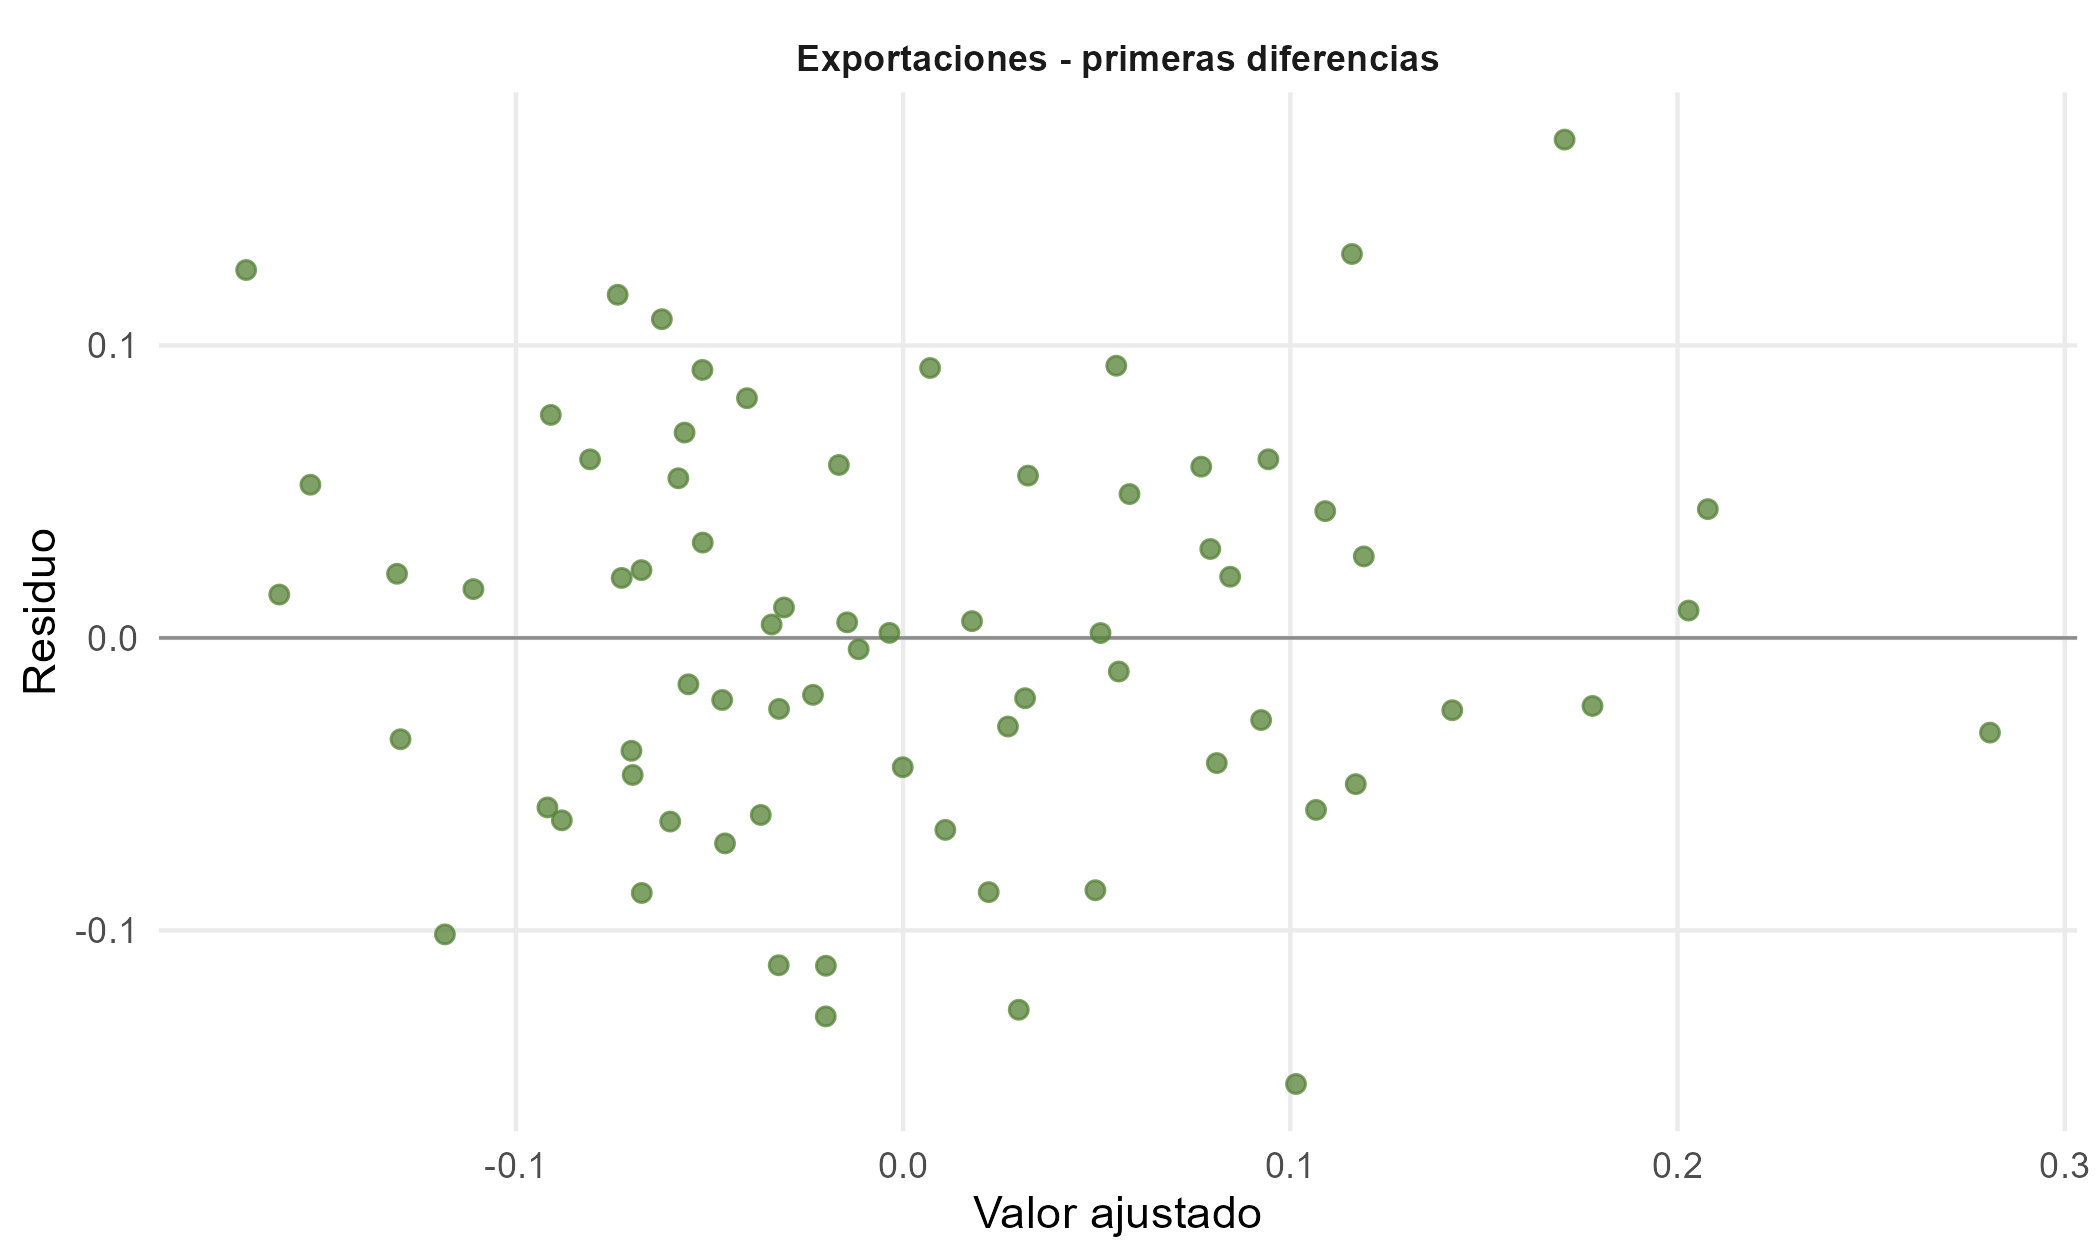
\includegraphics[width=0.82\textwidth]{section_12_fitted_vs_residuals_exports.png}
\caption{Valores ajustados y residuos del modelo de exportaciones.}
\label{fig:ajustados-vs-residuos-exportaciones}
\end{figure}

\begin{figure}[H]
\centering
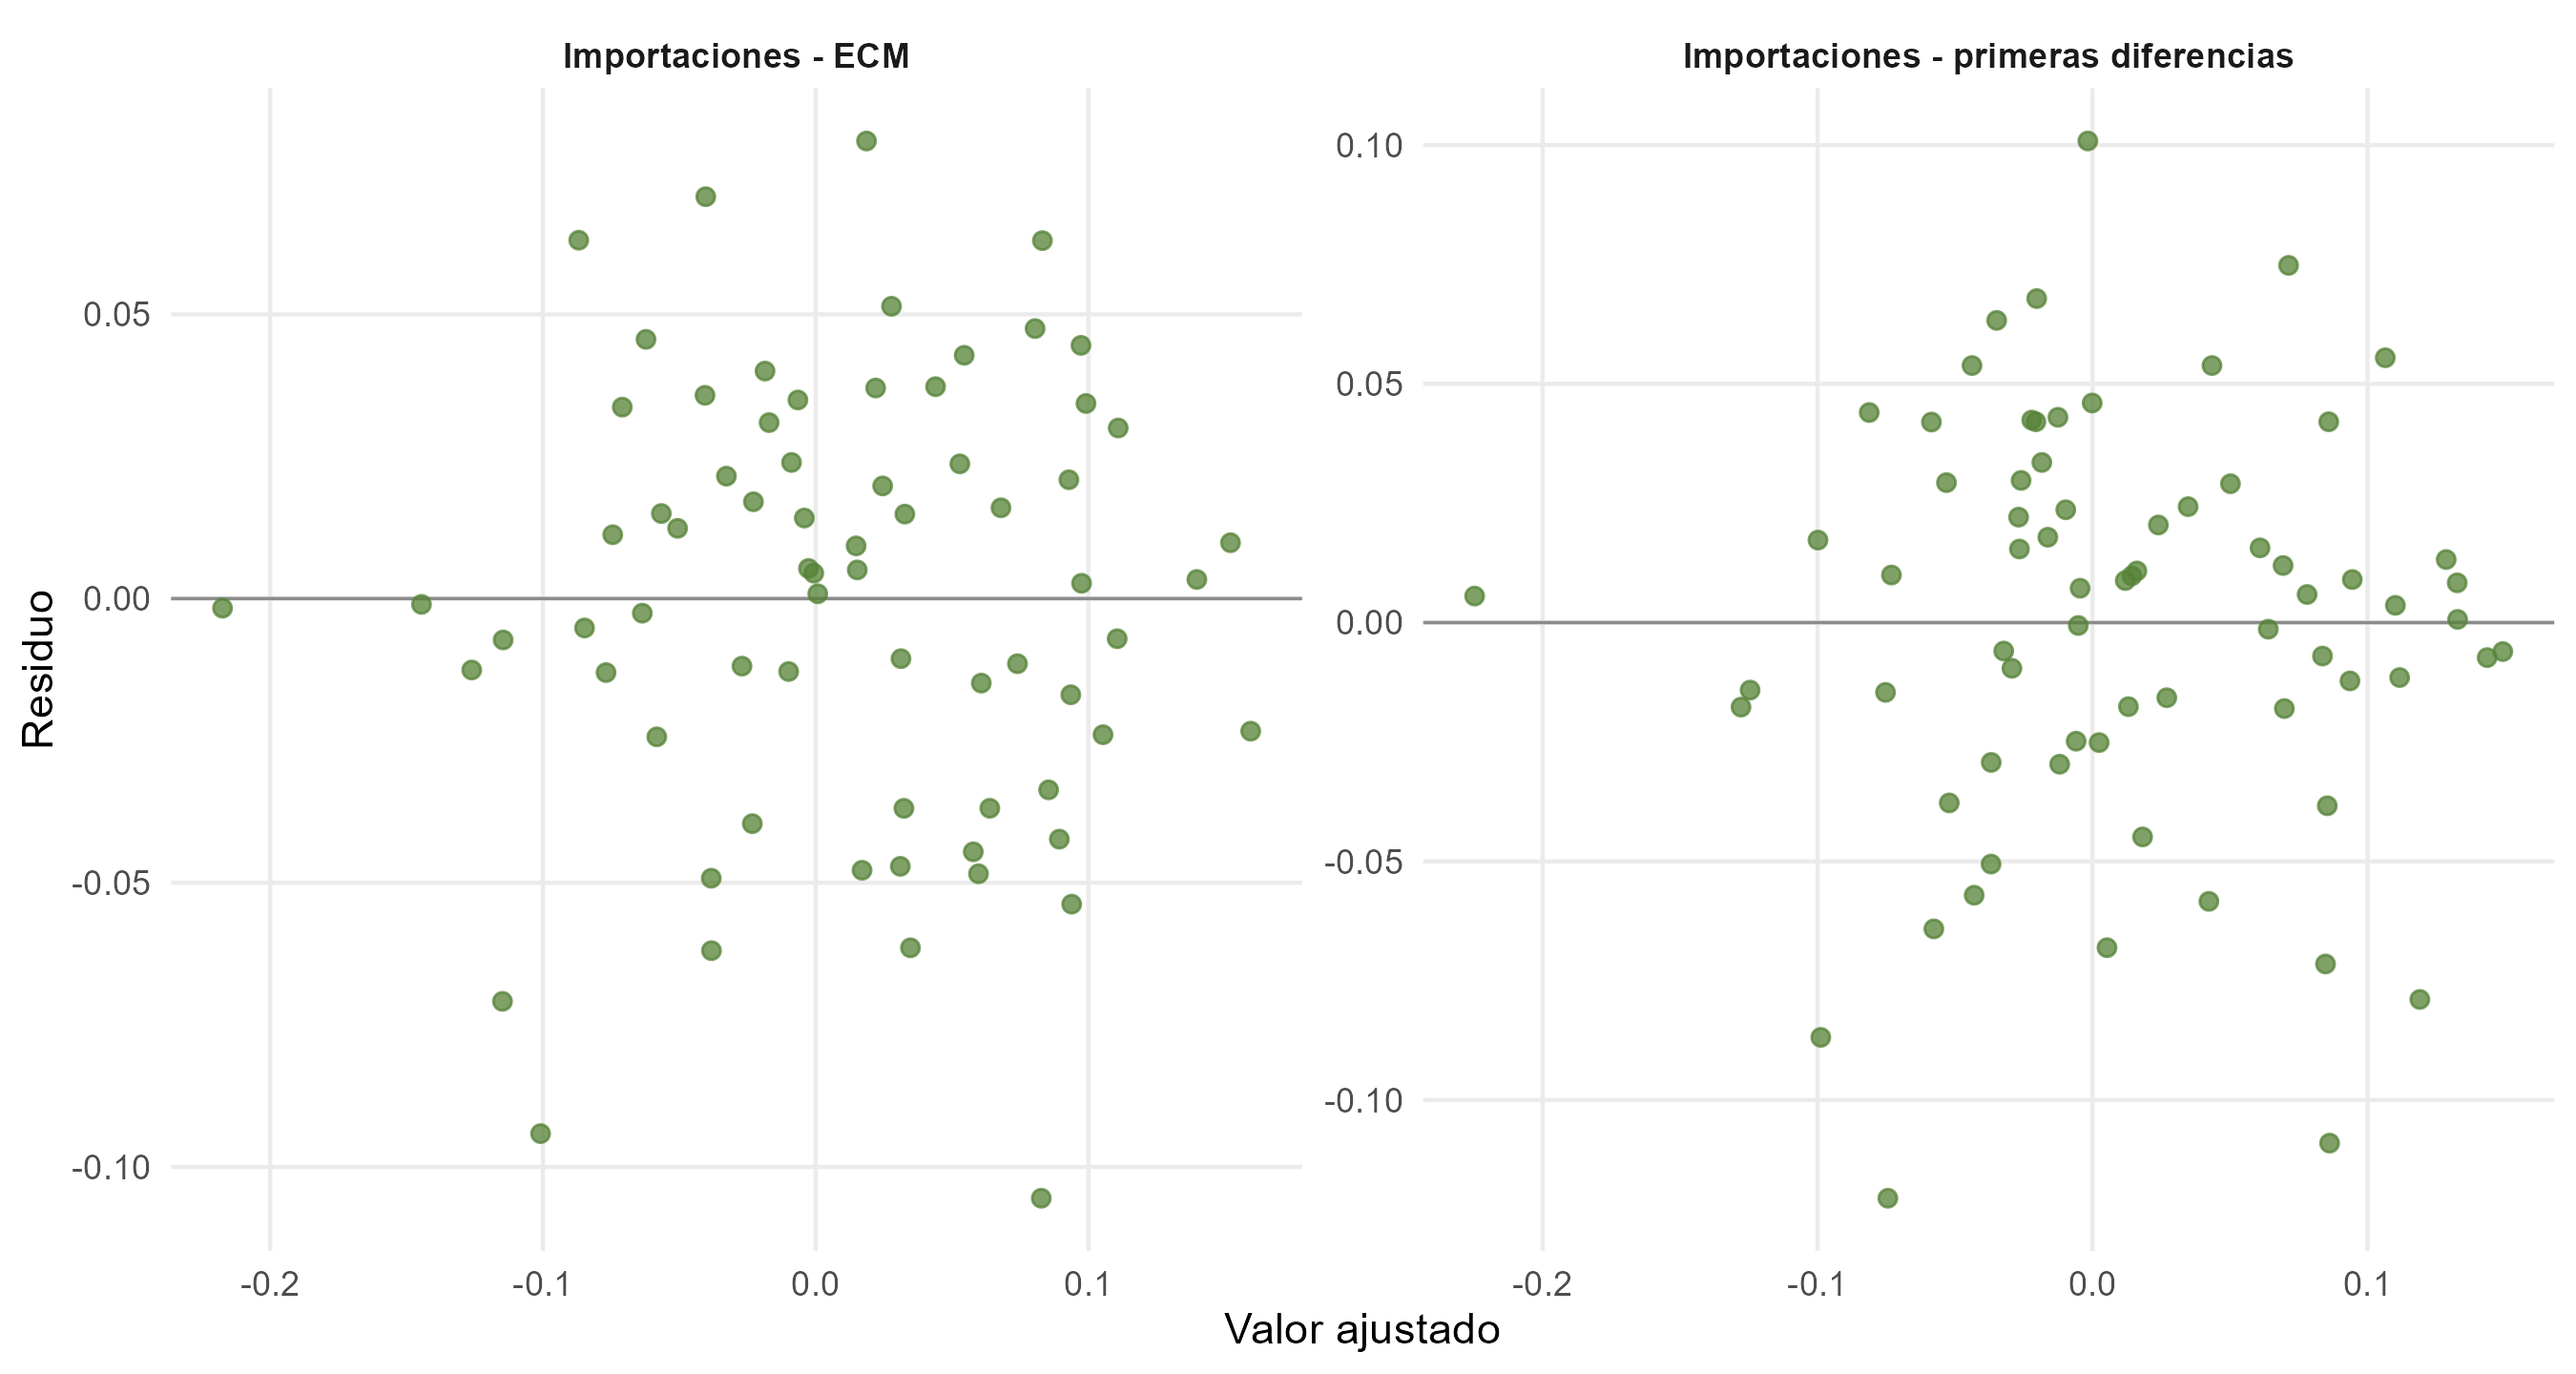
\includegraphics[width=\textwidth]{section_12_fitted_vs_residuals_imports.png}
\caption{Valores ajustados y residuos de los modelos de importaciones.}
\label{fig:ajustados-vs-residuos-importaciones}
\end{figure}
 		
% -------------------------------
% 6. Comparación de métodos
% -------------------------------
\section{Comparación de métodos}
\label{sec:comparacion-metodos}

\begin{table}[H]
\centering
\caption{Comparación preliminar con la literatura.}
\label{tab:comparacion-literatura}
\small
\resizebox{\textwidth}{!}{%
\begin{tabular}{llllll}
\toprule
Fuente & Período & Flujo & Horizonte & Elasticidad ingreso & Elasticidad tipo de cambio \\
\midrule
Este trabajo & 2004Q1--2022Q4 & Importaciones & Largo plazo & 1.518 & -0.399 \\
Este trabajo & 2004Q1--2022Q4 & Exportaciones & Largo plazo & 0.720 & 0.159 \\
Berrettoni y Castresana (2008) & Pendiente & Pendiente & Pendiente & Pendiente & Pendiente \\
Bus y Nicolini-Llosa (2007) & Pendiente & Pendiente & Pendiente & Pendiente & Pendiente \\
Zack y Sotelsek (2016) & Pendiente & Pendiente & Pendiente & Pendiente & Pendiente \\
\bottomrule
\end{tabular}%
}
\end{table}



% -------------------------------
% 7. Conclusiones
% -------------------------------
\section{Conclusiones}
\label{sec:conclusiones}



% -------------------------------
% Bibliografía
% -------------------------------
\begin{thebibliography}{9}



\end{thebibliography}


% -------------------------------
% Anexos
% -------------------------------
\appendix
\section{Anexos}
\label{sec:anexos}

\subsection{Trazabilidad y reproducibilidad}
\label{subsec:trazabilidad-reproducibilidad}

\begin{table}[H]
\centering
\caption{Checklist de reproducibilidad del script.}
\label{tab:checklist-reproducibilidad}
\footnotesize
\begin{tabular}{p{10.5cm}c}
\toprule
Control & Cumple \\
\midrule
Calendario trimestral 2004Q1--2025Q4 construido & Sí \\
Panel transformado con logs, diferencias, rezagos y PIBSOCIOS & Sí \\
Muestra econométrica común documentada & Sí \\
Estacionalidad evaluada en primeras diferencias & Sí \\
Series principales clasificadas como I(1) & Sí \\
Cointegración evaluada para importaciones y exportaciones & Sí \\
Residuos Engle-Granger incorporados al panel de modelación & Sí \\
Modelos ECM/diferencias estimados y exportados & Sí \\
Diagnósticos post-estimación sin alertas al 5\% & Sí \\
Outputs finales esperados disponibles & Sí \\
Trazabilidad de PIBSOCIOS disponible & Sí \\
\bottomrule
\end{tabular}
\end{table}

\begin{table}[H]
\centering
\caption{Índice final de salidas generadas por el script.}
\label{tab:indice-salidas}
\small
\begin{tabular}{lcc}
\toprule
Grupo de salida & Estado & Archivos \\
\midrule
Base & Disponible & 5 \\
Figura & Disponible & 9 \\
Tabla econométrica & Disponible & 4 \\
Trazabilidad & Disponible / generada por sección & 5 \\
Entrega & Disponible / pendiente externa al script & 3 \\
\bottomrule
\end{tabular}
\end{table}


\end{document}

